\chapter{Real-Time Pattern-Based Recognition on a Neuromorphic System}
\label{cha:pattern}

%\section{Hard-wired Network Model}
To explore how brain may recognise objects, we have employed a biologically-inspired DVS silicon retina~\cite{lenero20113}, a good example of low-cost visual processing due to its event-driven and redundancy-reducing style of computation;
and a SpiNNaker system~\cite{furber2014spinnaker}, which is a massive parallel computing platform aimed at real-time simulation of SNNs. 
%SpiNNaker, as the back-end of the system, provides a flexible, event-driven mechanism for real-time simulation of SNNs, and is where the posture recogniser locates.
With this neuromorphic hardware system we have the ability to explore visual processing by mimicking the functions of various regions along the visual pathway. 
Building a real-time recognition system for dynamic hand postures is a first step of exploring visual processing in a biological fashion and is also a validation of the neuromorphic platform.
To match the image properties detailed earlier, the position, shape, size and trajectory of the hand postures can be detected from the retina output.
To keep the task simple at first, the postures are of similar size and the goal is to recognise the shape of a hand with moving positions.
Tracking the postures with a short memory will form part of the future work.

Dynamic recognition takes advantage of the intrinsic temporal processing of SNNs which are receiving considerable attention for undertaking vision processing.
Pattern information can be encoded in the delays between the pre- and post-synaptic spikes since the spiking neurons are capable of computing radial basis functions (RBFs)~\cite{hopfield1995pattern}.
Spatio-temporal information can also be stored in the exact firing time rather than relative delays~\cite{natschlager1998spatial}.

\section{The Neuromorphic Platform}
\label{sec:np}
The outline of the platform is illustrated in Fig.~\ref{fig:SysOverViewa}, where the hardware system is configured, controlled and monitored by the PC.
%Fig.~\ref{fig:SysOverViewb} shows the combined hand posture recognition system; 
The jAER~\cite{delbruck2008frame} event-based processing software on the PC configures the retina and displays the output spikes through a USB link.
The host communicates to the SpiNNaker board via Ethernet to set up its runtime parameters and to download the neural network model off-line.
It visualises~\cite{6252490} the spiking activity of the network in real-time.
The photograph of the hardware platform, Fig.~\ref{fig:SysOverViewb}, shows that the silicon retina connects to the SpiNNaker 48-node system via a Spartan-6 FPGA board~\cite{galluppi2012real}.
%, which was also applied to a sound localisation system.


\begin{figure}
\centering
	\begin{subfigure}[t]{0.8\textwidth}
		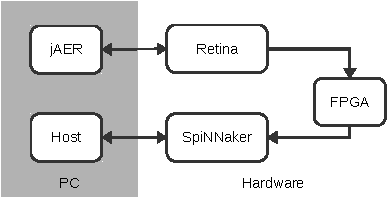
\includegraphics[width=\textwidth]{pics_icann/outline.pdf}
	    \caption{Outline of the platform.}
	    \label{fig:SysOverViewa}
	\end{subfigure}
	\\
	\begin{subfigure}[t]{0.8\textwidth}
		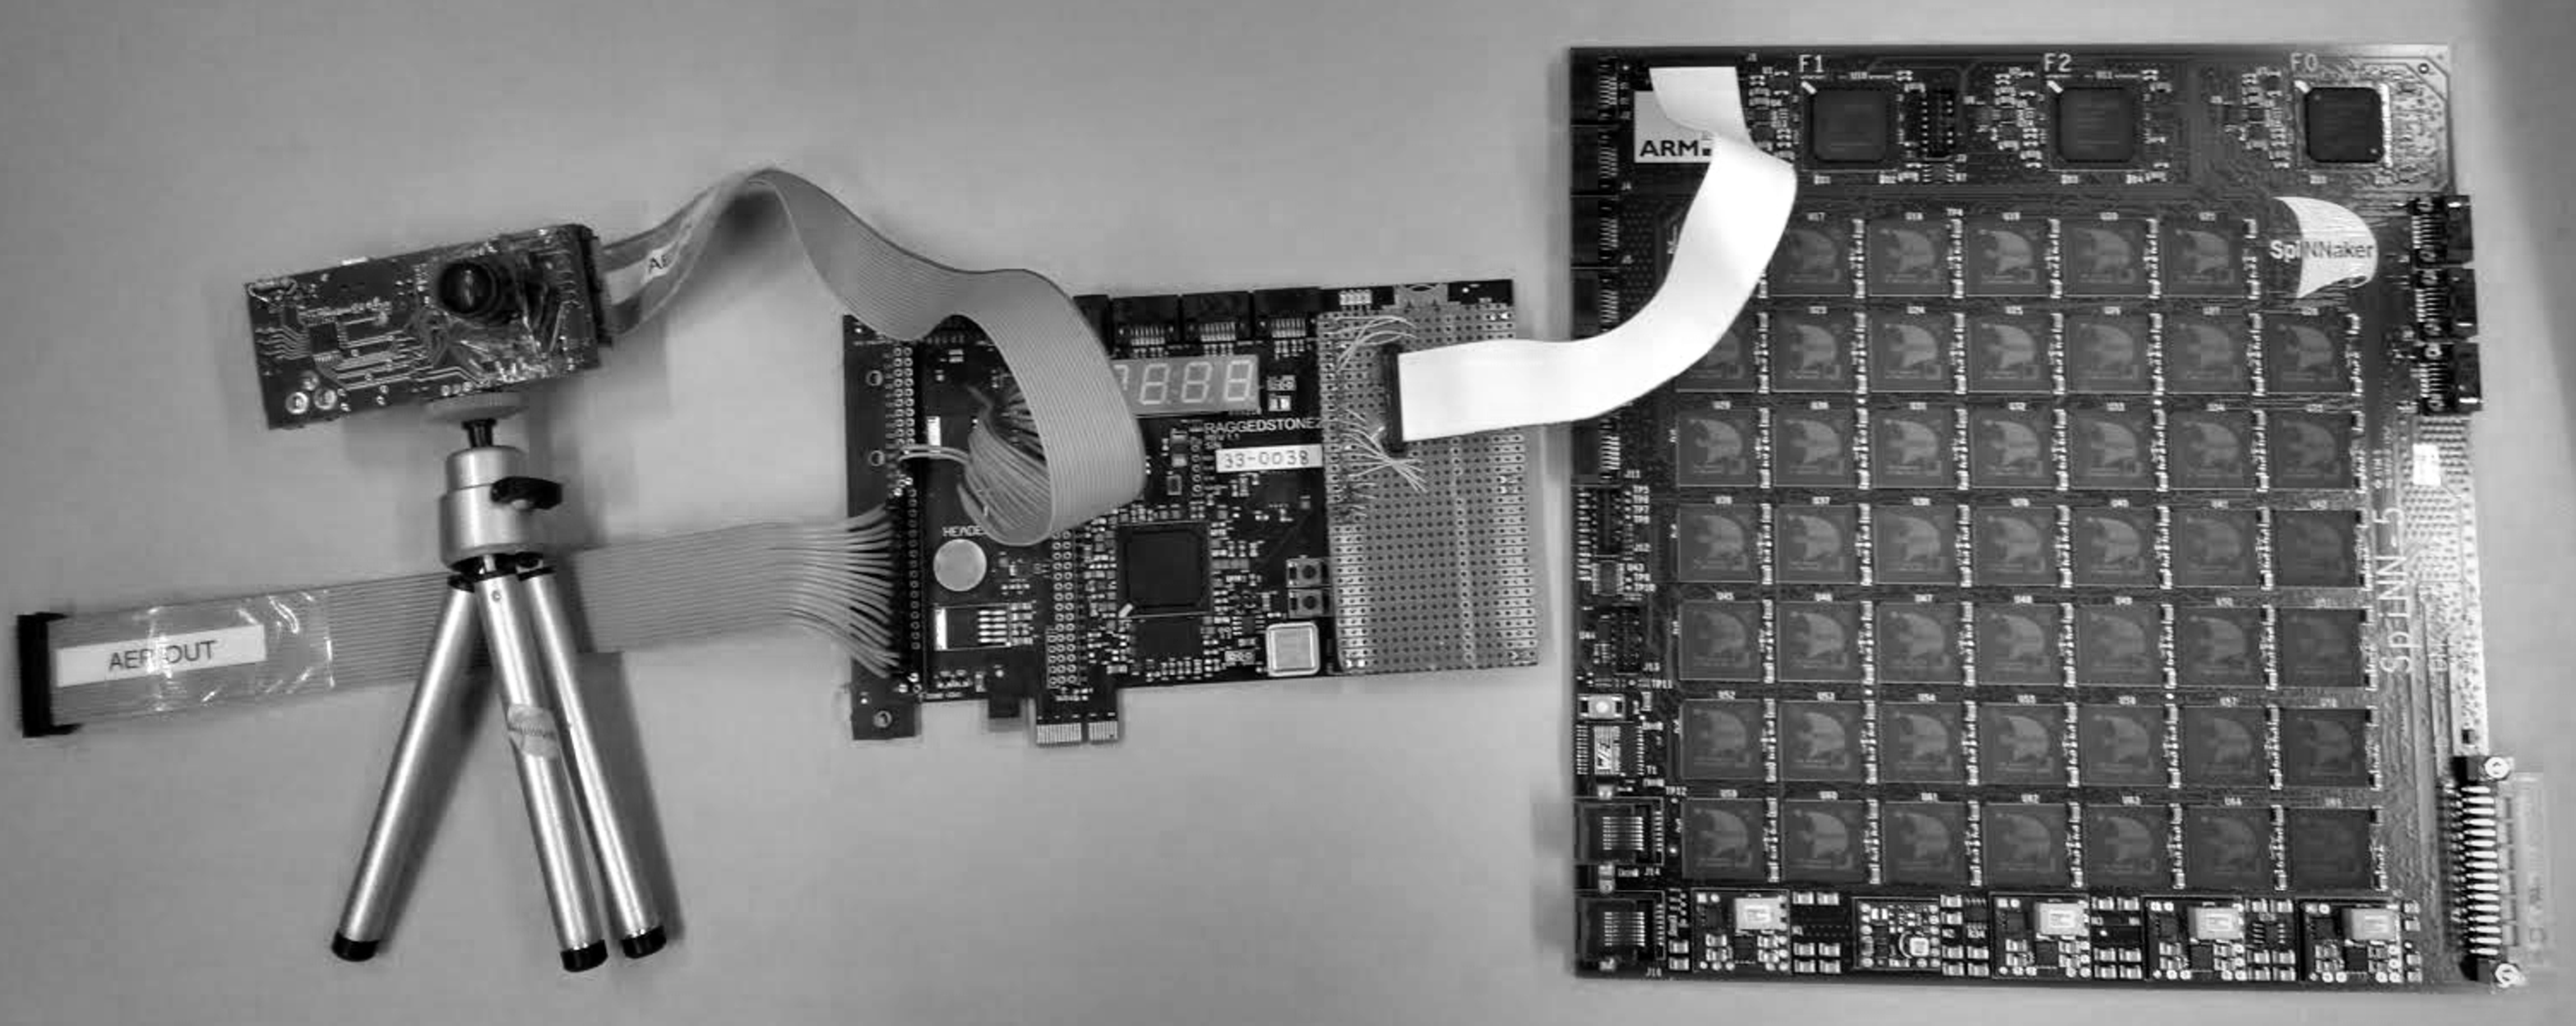
\includegraphics[width=\textwidth]{pics_icann/outline2.pdf}	    \caption{Picture of the hardware platform. From left to right: a silicon retina, a FPGA board, and a 48-node SpiNNaker system.}
	    \label{fig:SysOverViewb}
	\end{subfigure}	

\caption{System overview of the dynamic hand posture recognition platform. 
%The silicon retina connects to the SpiNNaker system through an FPGA board. 
%Spikes from the retina are streamed to the SpiNNaker system through this Spartan-6 FPGA board.
%The jAER software configures the retina and displays its outgoing spikes through the USB connection.
%The host sets up the runtime parameters off-line and downloads the network model to the SpiNNaker system.
}
\label{fig:SysOverView}
\end{figure}

\subsection{Silicon Retina}
The visual input is captured by a DVS silicon retina, which is quite different from conventional video cameras.
Each pixel generates spikes when its change in brightness reaches a defined threshold.
Thus, instead of buffering video into frames, the activity of pixels is sent out and processed continuously with time.
The communication bandwidth is therefore optimised by sending activity only, which is encoded as pixel events using Address-Event Representation (AER~\cite{lazzaro1995multi}) protocol.
The level of activity depends on the contrast change; pixels generate spikes faster and more frequently when they are subject to more active change.
The sensor is capable of capturing very fast moving objects (e.g., up to 10 K rotations per second), which is equivalent to 100 K conventional frames per second~\cite{lenero20113}.

\subsection{SpiNNaker System}
The SpiNNaker project's architecture mimics the human brain's biological structure and functionality. 
This offers the possibility of utilizing massive parallelism and redundancy, as the brain, to provide resilience in an environment of unreliability and failure of individual components.

In the human brain, communication between its computing elements, or neurons, is achieved by the transmission of electrical `spikes' along connecting axons. 
The biological processing of the neuron can be modelled by a digital processor and the axon connectivity can be represented by messages, or information packets, transmitted between a large number of processors which emulate the parallel operation of the billions of neurons comprising the brain.

The engineering of the SpiNNaker concept is illustrated in Fig.~\ref{fig:sysdia} where the hierarchy of components can be identified. 
Each element of the toroidal interconnection mesh is a multi-core processor known as the `SpiNNaker Chip' comprising 18 processing cores. 
Each core is a complete processing sub-system with local memory.
It is connected to its local peers via a Network-on-Chip (NoC) which provides high bandwidth on-chip communication and to other SpiNNaker chips via links between them. 
In this way massive parallelism extending to thousands or millions of processors is possible.

\begin{figure}
\centering
	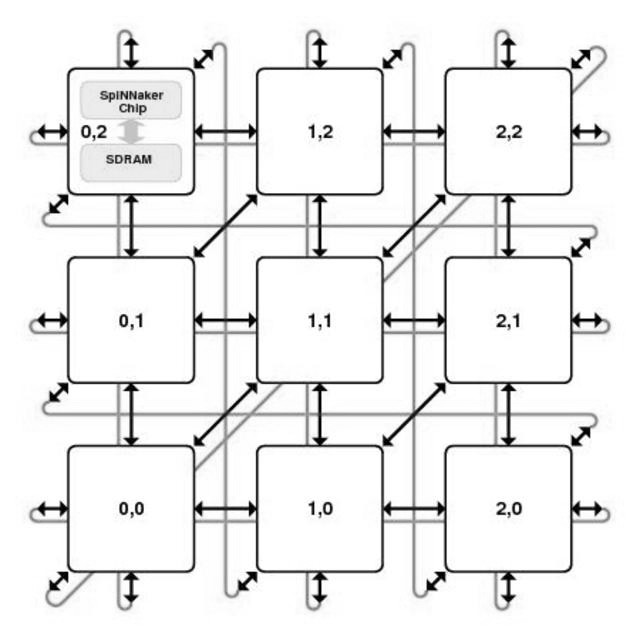
\includegraphics[width=0.7\textwidth]{pics_icann/mesh_ctiff.jpg}
	\caption{SpiNNaker system diagram.
	Each element represents one chip with local memory.
	Every chip connects to its neighbours through the six bi-directional on-board links. }
	\label{fig:sysdia}
\end{figure}

%The knowledge content and learning ability of the brain is generally thought to be embodied in its evolvable interconnection pattern.
%This structure routes a spike generated by one neuron to others which are interconnected with it via axons and these interconnections are modified and extended as a result of learning processes.
%
%In SpiNNaker a packet router within each multi-core processor controls the neural interconnection. 
%Each transmitted packet represents a spike and simply identifies its source neuron.
%This is used by routers to identify whether a packet should be routed to a processor core, or should be routed on to one of the six adjacent chips connected to it as part of the overall SpiNNaker network.

The `103 machine' is the name given to the 48-node board which we use for the hand posture recognition system, see Fig.~\ref{fig:SysOverViewb}.
It has 864 ARM processor cores, typically deployed as 768 application, 48 monitor and 48 spare cores. 
%The `103 machine' requires a 12V 6A supply. 
%The control interface is via two 100Mbps Ethernet connections, one for the board management processor and the second for the SpiNNaker array. 
%There are options to use the nine on-board 3.0~Gbps high-speed serial interfaces (using SATA cables, but not necessarily the SATA protocol) for I/O; 
%this will require suitable configuration of the on-board FPGAs that provide the high-speed serial interface support. 
The boards can be connected together to form larger systems using high-speed serial interfaces. 

%\begin{figure}
%\centering
%	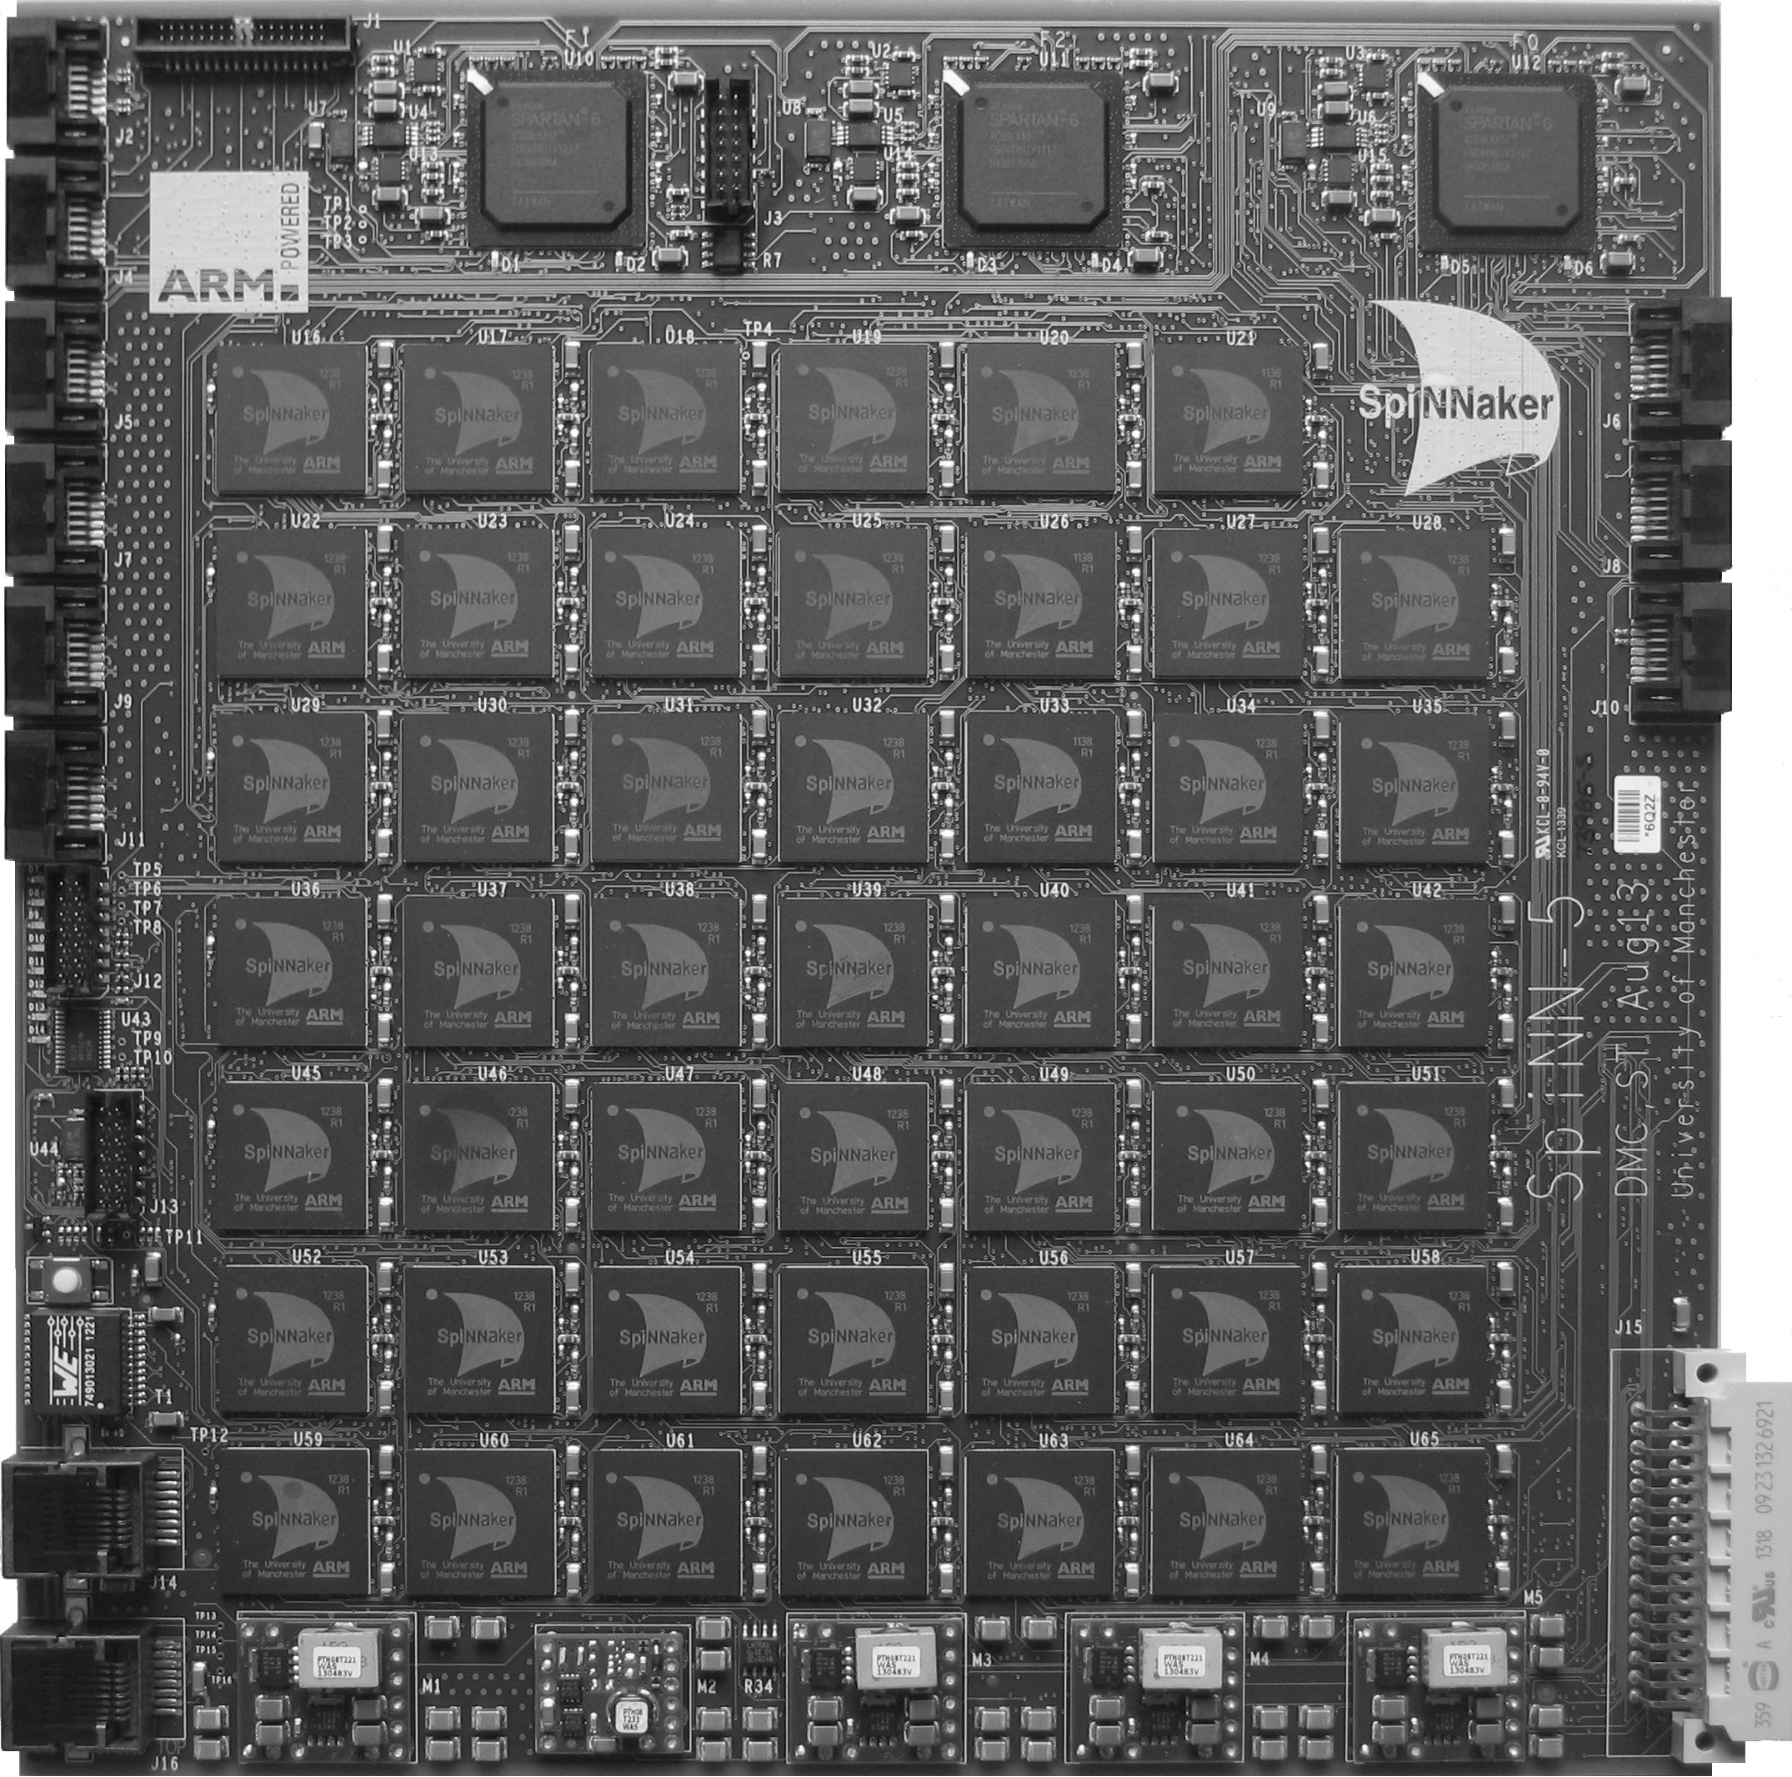
\includegraphics[width=0.42\textwidth]{pics_icann/SpiNN5.pdf}
%	\caption{`103 Machine' PCB}
%	\label{fig:48node}
%\end{figure}

\subsection{Interfacing AER Sensors}
Spikes from the silicon retina are injected directly into SpiNNaker via a SPARTAN-6 FPGA board that translates them into a SpiNNaker compatible AER format~\cite{appnote8}. 

From a neural modelling point of view, interfacing the silicon retina is performed using pyNN~\cite{davison2008pynn}. 
The retina is configured as a spike source population that resides on a virtual SpiNNaker chip, to which an AER sensor's spikes are directed, thus abstracting away the hardware details from the user\cite{galluppi2012real}.
Besides the retina, we have successfully connected an AER based silicon cochlea~\cite{5537164} to SpiNNaker for a sound localisation task~\cite{6706931}.

\section{Methods}
The convolutional network is well-known as an example of a biologically-inspired model. 
Fig.~\ref{fig:conv} shows a typical convolutional connection between two layers of neurons. 
The repeated convolutional kernels are overlapped in the receptive fields of the input neurons. 
\begin{figure}
\centering
	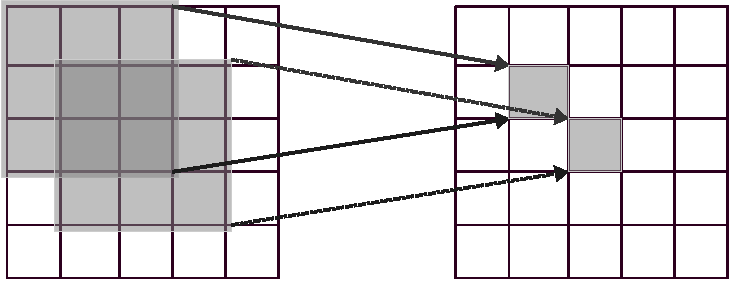
\includegraphics[width=0.7\textwidth]{pics_icann/conv.pdf}
	\caption{Each individual neuron in the convolution layer (right matrix) connects to its receptive field using the same kernel. The value of the kernel is represented by the synaptic weights between the connected neurons.}
	\label{fig:conv}
\end{figure}

There are two CNNs proposed to accomplish the dynamic hand posture recognition task.
A straight forward method of template matching is employed at first, followed by a network of multi-layer perceptrons (MLP) trained to improve the recognition performance.


\begin{figure}
\centering
	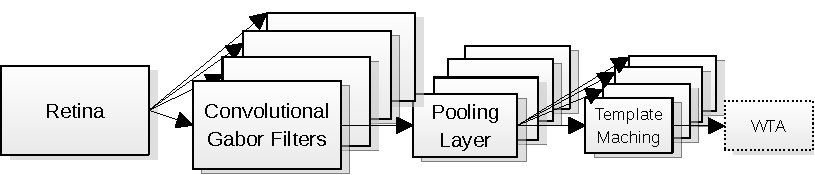
\includegraphics[width=0.9\textwidth]{pics_icann/model1.pdf}
	\caption{Model 1. 
	The retina input is convolved with Gabor filters in the second layer, and then shrinks the sizes in the pooling layer.
	The templates are considered as convolution kernels in the last layer.
	The WTA circuit can be used as an option to show the template matching result more clearly.
	}
	\label{fig:model1}
\end{figure}
%\subsubsection{Model 1. Template Matching}

Model 1: Template Matching. Shown in Fig.~\ref{fig:model1} the first layer is the retina input, followed by the convolutional layer, where the kernels are Gabor filters responding to edges of four orientations.
The third layer is the pooling layer where the size of the populations shrinks. 
This down-sampling enables robust classification due to its tolerance to variations in the precise shape of the input. 
The fourth layer is another convolution layer where the output from the pooling layer is convolved with the templates.
The optional layer of Winner-Take-All (WTA) neurons enables a clearer classification result due to the inhibition between the neurons.
In the Matlab simulation, the retina input spikes are buffered into 30~ms frames, and the neurons are simple linear perceptrons.
The templates are chosen by sampling the output of the pooling layer when given some reference stimulus, see Fig.~\ref{fig:template}.

\begin{figure}
\centering
	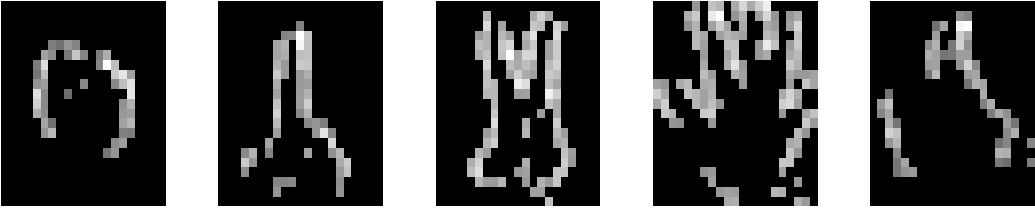
\includegraphics[width=0.9\textwidth]{pics_icann/gesture.pdf}
	\caption{Templates of the five postures: `Fist',`Index Finger', `Victory Sign', `Full Hand' and `Thumb up'.}
	\label{fig:template}
\end{figure}

The Gabor filter is well-known as a linear filter for edge detection in image processing. 
A Gabor filter is a 2D convolution of a Gaussian kernel function and a sinusoidal plane wave; see~(\ref{equ:gabor}). 
\begin{equation}
\begin{array}{l}
\mathrm{Real Parts} = \exp \left(\frac{-x^{'2}+y^{'2}}{2\sigma ^{2}}\right)\cos \left(2\pi\frac{{x}'}{\lambda }\right)
\\
\\
\mathrm{Imaginary Parts} = \exp \left(\frac{-x^{'2}+y^{'2}}{2\sigma ^{2}}\right)\sin \left(2\pi\frac{{x}'}{\lambda }\right)
\\
\\
\mathrm{where:}
\\
\\
{x}'=x\cos (\theta ) + y\sin (\theta)
\\
\\
{y}'=-x\sin (\theta ) + y\cos (\theta)
\end{array}
\label{equ:gabor}
\end{equation}
$\theta$ represents the orientation of the filter, $\lambda$ is the wavelength of the sine wave, and $\sigma$ is the standard deviation of the Gaussian envelope. 
The frequency and orientation features are similar to the responses of V1 neurons in the human visual system. 
Only the real parts of the Gabor filters (see Fig.~\ref{fig:gabor}) are used as the convolutional kernels to configure the weights between the input layer and the Gabor filter layer.

\begin{figure}
\centering
	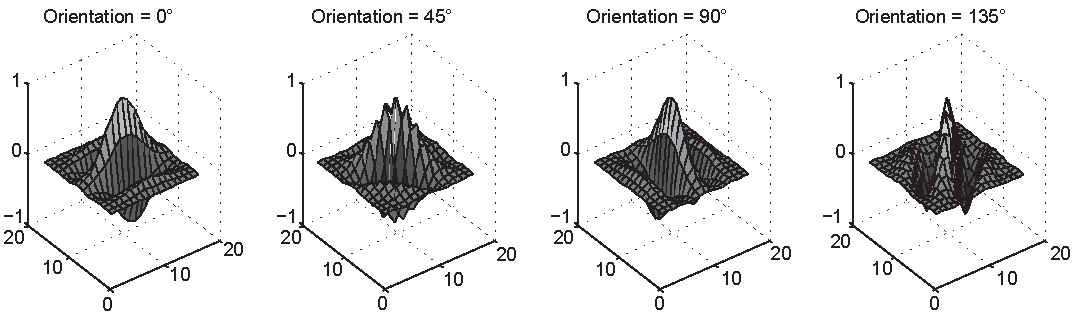
\includegraphics[width=0.9\textwidth]{pics_icann/gabor.pdf}
	\caption{Real parts of the Gabor filters orienting four directions.}
	\label{fig:gabor}
\end{figure}

%The templates (see Fig.~\ref{fig:template}) are manually selected from the output of the pooling layer in the framed Matlab simulation. 
The output score of a convolution is determined by the matching degree between the input and the kernel.
Regarding the template matching layer, each neuron in a population responds to how closely its receptive field matches the specific template.
The position of moving gesture is also naturally encoded in the address of template matching neuron.
Thus, there are five populations of template matching neurons, one for each hand posture listed.

%\subsubsection{Model 2. Trained MLP}
Model 2: Trained MLP. 
Inspired by the research of Lecun~\cite{lecun1998gradient}, we designed a combined network model with MLP and CNN (Fig.~\ref{fig:model2}). 
The first three layers are exactly the same as the previous model.
The training images for the 3-layered MLP are of same size and the posture is centred in the images.
Therefore, a tracking layer plays an important role to find the most active region and forward the centred image to the next layer.

\begin{figure}
\centering
	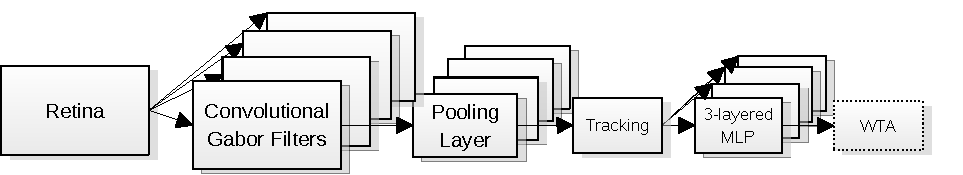
\includegraphics[width=0.9\textwidth]{pics_icann/model2.pdf}
	\caption{Model 2. 
	The retina input convolves with Gabor filters in the second layer, and then shrinks the sizes in the pooling layer.
	The following tracking layer finds the most active area of some fixed size, moves the posture to the centre and pushes the image to the trained MLP.
	The winner-take-all (WTA) layer can be used as an option to show the template matching result more clearly.}
	\label{fig:model2}
\end{figure}

%Since the size of the input image of the MLP training is fixed and the position is centered, tracking plays a very important role to spot the valid region. 
%Tracking is naturally embedded in the pooling layer of the convolutional network, for the active neurons directly point out the lively receptive field. 

\section{Results}

In order to evaluate the cost and performance trade-offs in optimizing the number of neural components, both the convolutional models described above are tested at different scales. 
Five videos of every posture are captured from the silicon retina in AER format, all of similar size and moving clock-wise in front of the retina. 
The videos are cut into frames (30~ms per frame) and presented to the convolutional networks. 
The configurations of the networks are listed in Table~\ref{tbl:nns}.
The integration layer is not necessary in a convolutional network, but is used here to decrease the number of synaptic connections.

\begin{table}
\caption{Sizes of the convolutional neural networks.}
	\begin{subtable}{0.8\textwidth}
		
		\centering
		\caption{Model 1: Template matching}
		\begin{tabular}{p{0.26\textwidth}|p{0.3\textwidth}<{\centering}|p{0.26\textwidth}<{\centering}|p{0.26\textwidth}<{\centering}|p{0.26\textwidth}<{\centering}}
		%Line 1
		\Xhline{1.2pt}
		    & \multicolumn{2}{c|}{\tabincell{c}{\textbf{Full Resolution } \\\textbf{128 $\times$ 128}}}  
		    & \multicolumn{2}{c}{\tabincell{c}{\textbf{Sub-sampled Resolution} \\\textbf{32 $\times$ 32}}}
		    \\ \cline{2-5}
		%Line 2
			& \tabincell{c}{Population \\ Size}
			& \tabincell{c}{Connections \\ per Neuron}
			& \tabincell{c}{Population \\ Size}
			& \tabincell{c}{Connections \\ per Neuron}
			\\ \Xhline{1.2pt}
		%Line 3
		\tabincell{l}{\textbf{Retinal} \\\textbf{Input}}
			& 128 $\times$ 128	& 1	& 32 $\times$ 32	& 4 $\times$ 4
			\\ \hline
		%Line 4
		\tabincell{l}{\textbf{Gabor} \\\textbf{Filter}}
			& 112$\times$112$\times$4	& 17 $\times$ 17	& 28$\times$28$\times$4	& 5 $\times$ 5
			\\ \hline
		%Line 5
		\tabincell{l}{\textbf{Pooling} \\\textbf{Layer}}
			& 36$\times$36$\times$4	& 5 $\times$ 5	& null	& null
			\\ \hline
		%Line 6
		\tabincell{l}{\textcolor[rgb]{0.55,0.55,0.55}{\textbf{Integration}} \\ \textcolor[rgb]{0.55,0.55,0.55}{\textbf{Layer}}}
			& 36 $\times$ 36	& 4	& 28 $\times$ 28	& 4
			\\ \hline
		%Line 7
		\tabincell{l}{\textbf{Template} \\\textbf{Matching}}
			& 16$\times$16$\times$5	& 21 $\times$ 21	& 14$\times$14$\times$5	& 15 $\times$ 15
			\\ \Xhline{1.2 pt}
		%Line 8
		\textbf{Total}
			& $74,320$	& $15,216,512$	& $5,925$	& $318,420$
			\\ \Xhline{1.2 pt}
		\end{tabular}
		\label{tbl:m1}
	\end{subtable}
	\par\bigskip
	\begin{subtable}{0.8\textwidth}
		
		\centering
		\caption{Model 2: Trained MLP}
		\begin{tabular}{p{0.26\textwidth}|p{0.30\textwidth}<{\centering}|p{0.26\textwidth}<{\centering}|p{0.26\textwidth}<{\centering}|p{0.26\textwidth}<{\centering}}
		%Line 1
		\Xhline{1.2pt}
		    & \multicolumn{2}{c|}{\tabincell{c}{\textbf{Full Resolution} \\\textbf{128 $\times$ 128}}}  
		    & \multicolumn{2}{c}{\tabincell{c}{\textbf{Sub-sampled Resolution} \\\textbf{32 $\times$ 32}}}
		    \\ \cline{2-5}
		%Line 2
			& \tabincell{c}{Population \\ Size}
			& \tabincell{c}{Connections \\ per Neuron}
			& \tabincell{c}{Population \\ Size}
			& \tabincell{c}{Connections \\ per Neuron}
			\\ \Xhline{1.2pt}
		%Line 3
		\tabincell{l}{\textbf{Tracked} \\\textbf{Input}}
			& 21 $\times$ 21	& null	& 15 $\times$ 15	& null
			\\ \hline
		%Line 4
		\tabincell{l}{\textbf{Hidden} \\\textbf{Layer}}
			& 10	& 21$\times$21$\times$10	& 10	& 15$\times$15$\times$10
			\\ \hline
		%Line 5
		\tabincell{l}{\textbf{Recognition} \\\textbf{Layer}}
			& 5	& 5$\times$10	& 5	& 5$\times$10
			\\ \Xhline{1.2pt}
		%Line 6
		\textbf{Total}
			& $456$	& $4,460$	& $240$	& $2,300$
			\\ \Xhline{1.2 pt}
		\end{tabular}
		\label{tbl:m2}
	\end{subtable}
	\label{tbl:nns}
\end{table}

\begin{figure}
\centering
	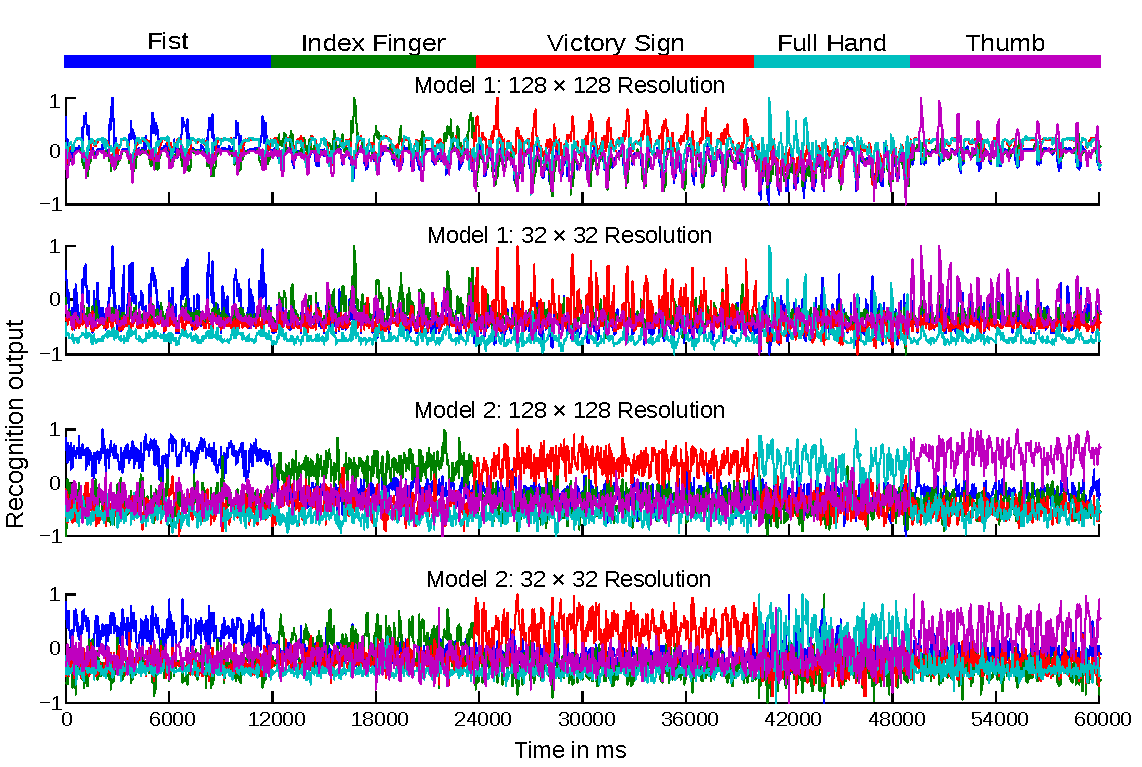
\includegraphics[width=\textwidth]{pics_icann/rateMatlab.pdf}
	\caption{Neural responses with time of four experiments to the same recorded moving postures.
	The recognition output is normalised to \mbox{[-1, 1]}.
	Every point represents the highest response in a specific population (different colour) for a 30~ms frame.
	The 1st plot refers to Model 1 with the full input resolution, and the 2nd plot Model 1 with the sub-sampled input resolution; and the 3rd and fourth plots both refer to Model 2, and with high and low input resolution respectively. 
	}
	\label{fig:matlabrec}
\end{figure}




In Fig.~\ref{fig:matlabrec} the first two plots refer to Model 1, using template matching. Each colour represents one of the recognition populations. 
Each point in the plot is the highest neuronal response in the recognition population during the time of one frame (30~ms). 
The neuronal response, `the spiking rate', is normalised to [-1, 1]. 
It can be seen that the higher resolution input makes the boundaries between the classes clearer. 
On the other hand, recognition only happens when the test image and template are similar enough. 
The templates are only selected from the frames where the gestures are moving towards the right, and the gestures are moving clockwise in the videos, thus, all the peaks in plot 1 correspond with moments when the gesture moves towards right.  
It is notable that the higher resolution causes the recogniser to be more sensitive to the differences between the test data and the template, while the smaller neural network can recognize more generalized patterns. 
Therefore, a threshold is required to differentiate between data that is close enough and that which is not. 
Since the gestures are moving in four different directions during the clockwise movement, a rejection rate (i.e. none of the template is matched) of 75\% is to be expected. 

The latter two plots of Fig.~\ref{fig:matlabrec} refer to Model 2. 
The three-layer MLP network significantly improves the recognition rate and can generalise the pattern. 
There is no rejection rate for Model 2, since the MLP is trained with all the moving directions of the postures.

Detailed results are listed in Table~\ref{tbl:rsl}. 
The correct recognition rate is calculated from the non-rejected frames.
The lower resolution of the 32$\times$32 retina input is adequate (85.83\%) for this gesture recognition task. 
The smaller network uses only 1/10th the number of neurons and 1/50th the number of synaptic connections compared with the full resolution network, while the recognition rate drops only around by 9.0\% with Model 1 and 17.2\% with Model 2.

\begin{table}
\centering
\caption{Recognition results using linear perceptrons in \%}
	\begin{tabular}{p{0.15\textwidth}|p{0.10\textwidth}<{\centering}|p{0.11\textwidth}<{\centering}|p{0.11\textwidth}<{\centering}|p{0.11\textwidth}<{\centering}|p{0.11\textwidth}<{\centering}}
		%Line 1
		\Xhline{1.2pt}
		    \multicolumn{2}{c|}{}	& \multicolumn{2}{c|}{\textbf{Model 1}}  
		    & \multicolumn{2}{c}{\textbf{Model 2}}
		    \\ \cline{3-6}
		%Line 2
		\multicolumn{2}{c|}{}	& \tabincell{c}{High \\ Resolution}
			& \tabincell{c}{Low \\ Resolution}
			& \tabincell{c}{High \\ Resolution}
			& \tabincell{c}{Low \\ Resolution}
			\\ \Xhline{1.2pt}
		%Line 3-4	
		\multirow{2}{*}{\tabincell{l}{\textbf{Fist}\\ (399 Frames)}}
			& Correct & 99.11	& 99.23	& 96.24	& 84.21
			\\ \cline{2-6}
			& Reject  & 71.93 & 67.42 	& Null	& Null
			\\ \hline
		%Line 5-6
		\multirow{2}{*}{\tabincell{l}{\textbf{Index Finger} \\ (392 Frames)}}
			& Correct & 92.98	& 80.00	& 94.39	& 71.69
			\\ \cline{2-6}
			& Reject & 70.92	& 75.77 	& Null	& Null
			\\ \hline
		%Line 7-8
		\multirow{2}{*}{\tabincell{l}{\textbf{Victory Sign} \\ (551 Frames)}}
			& Correct & 96.56	& 93.07	& 95.64	& 87.66
			\\ \cline{2-6}
			& Reject & 73.68	& 81.67 	& Null	& Null
			\\ \hline
		%Line 9-10
		\multirow{2}{*}{\tabincell{l}{\textbf{Full Hand} \\ (293 Frames)}}
			& Correct & 95.65	& 72.41	& 93.52	& 72.01
			\\ \cline{2-6}
			& Reject & 92.15	& 90.10 	& Null	& Null
			\\ \hline
		%Line 10-11
		\multirow{2}{*}{\tabincell{l}{\textbf{Thumb up} \\ (391 Frames)}}
			& Correct & 89.61	& 84.44	& 96.68	& 74.68
			\\ \cline{2-6}
			& Reject & 80.31	& 76.98 	& Null	& Null
			\\ \hline\hline
		\multirow{2}{*}{\tabincell{l}{\textbf{Average}}}
			& Correct & 94.78	& 85.83	& 95.29	& 78.05
			\\ \cline{2-6}
			& Reject & 77.80	& 78.39 	& Null	& Null
			\\ \hline
	\end{tabular}
	\label{tbl:rsl}
\end{table}

\section{Real-Time Recognition on SpiNNaker}
\subsection{Live Recognition}
We implemented the prototype of the dynamic posture recognition system on SpiNNaker using LIF neurons. 
The input retina layer consists of 128$\times$128 neurons; 
each Gabor filter has 112$\times$112 valid neurons, since the kernel size is 17$\times$17; 
each pooling layer is as big as 36$\times$36, convolving with five template kernels (21$\times$21); 
thus, the recognition populations are 16$\times$16 neurons each. Altogether $74,320$ neurons and $15,216,512$ synapses, use up to 19 chips (290 cores) on a 48-node board, see Table~\ref{tbl:m1}. Regarding the lower resolution of 32$\times$32 retinal input, the network (Table~\ref{tbl:m2}) consists of $5,925$ neurons and $318,420$ synapses taking up only two chips (31 cores) of the board.

Fig.~\ref{fig:live} shows snapshots of neural responses of some populations during real-time recognition.
Fig.~\ref{fig:live1} is a snapshot of the Gabor population which prefers the horizontal direction, given the input posture of a `Fist';
and Fig.~\ref{fig:live2} shows the activity of the neurons in the integration layer, given a 'Victory Sign'.
And the active neurons in the visualiser in Fig.~\ref{fig:live3} are pointing out the position of the recognised pattern the `Index finger'. 
All the supporting demonstrative videos can be found on YouTube~\cite{video1, video2, video3}. %\footnote{\url{
%https://www.youtube.com/watch?v=PvJy6RKAJhw&feature=youtu.be&list=PLxZ1W-Upr3eoQuLxq87qpUL-CwSphtEBJ, http://youtu.be/FZJshPCJ1pg?list=PLxZ1W-Upr3eoQuLxq87qpUL-CwSphtEBJ, http://youtu.be/yxN90aGGKvg?list=PLxZ1W-Upr3eoQuLxq87qpUL-CwSphtEBJ}}.

\begin{figure}
\centering
	\begin{subfigure}[t]{0.48\textwidth}
		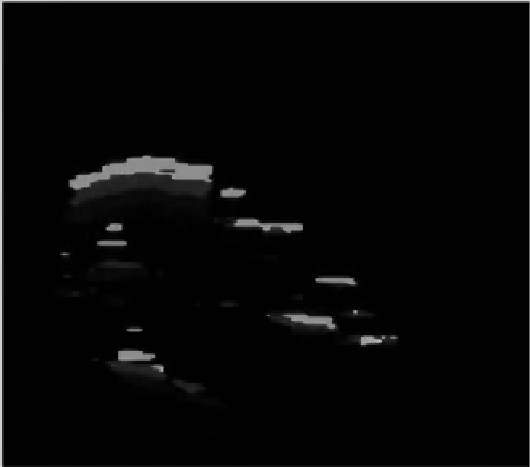
\includegraphics[width=\textwidth]{pics_icann/live1.png}
	    \caption{Neural responses of the Gabor filter layer orienting to the horizontal direction~\cite{video1} }
	    \label{fig:live1}
	\end{subfigure}
	\begin{subfigure}[t]{0.48\textwidth}
		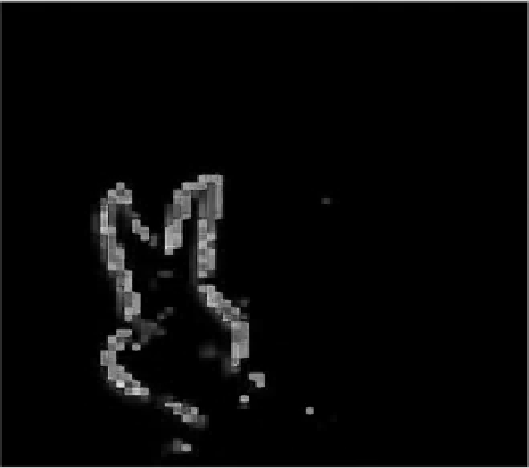
\includegraphics[width=\textwidth]{pics_icann/live2.png}
		\caption{Neural responses of the integrate layer~\cite{video2}}
	    \label{fig:live2}
	\end{subfigure}
	\\
	\begin{subfigure}[t]{0.80\textwidth}
		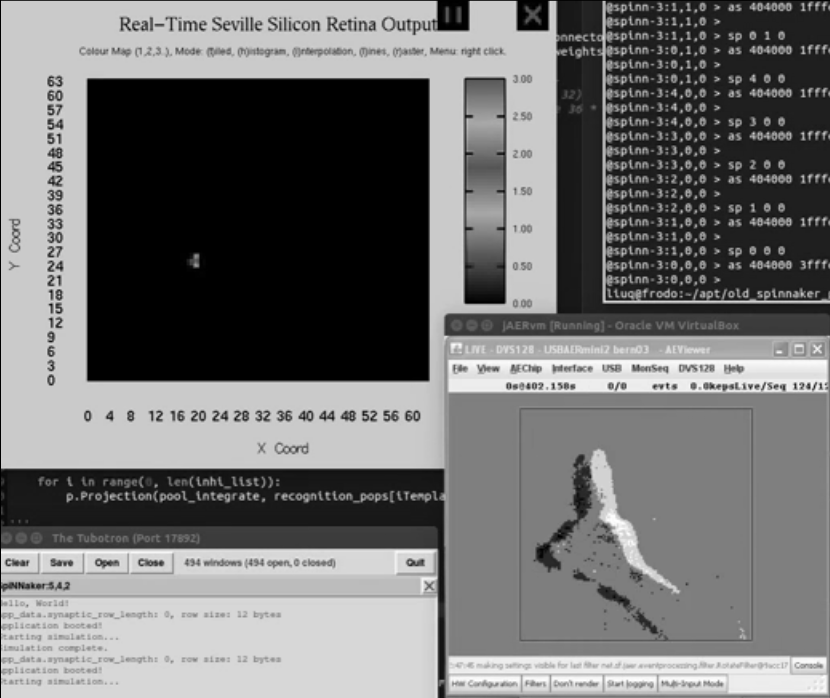
\includegraphics[width=\textwidth]{pics_icann/live.png}
		\caption{Snapshot of the neuron responses of the template matching layer~\cite{video3}}
	    \label{fig:live3}
	\end{subfigure}	

\caption{Snapshots of the real-time dynamic posture recognition system on SpiNNaker.
}
\label{fig:live}
\end{figure}

\subsection{Recognition of Recorded Data}
To compare with the results of the experiments carried out with Matlab (in Section~\ref{sec:exp}), the same recorded retinal data is conducted into SpiNNaker.
Only Model 1 is tested on the neuromorphic hardware platform, since tracking is still need to investigate using SNN (for Model 2) in the future. 
The recorded data is presented as spike source array in the system with 128$\times$128 input (see Fig.~\ref{fig:ssa}) while the data is forwarded to a sub-sampling layer of 32$\times$32 resolution in the system of the smaller network (see Fig.~\ref{fig:ssa32}). 
The output spikes generated from the recognition populations with time are shown in Fig.~\ref{fig:rps} and \ref{fig:rps32} for full resolution and lower systems respectively. 
More spikes are generated during the period when the preferred input posture is shown. 


\begin{figure}
\centering
	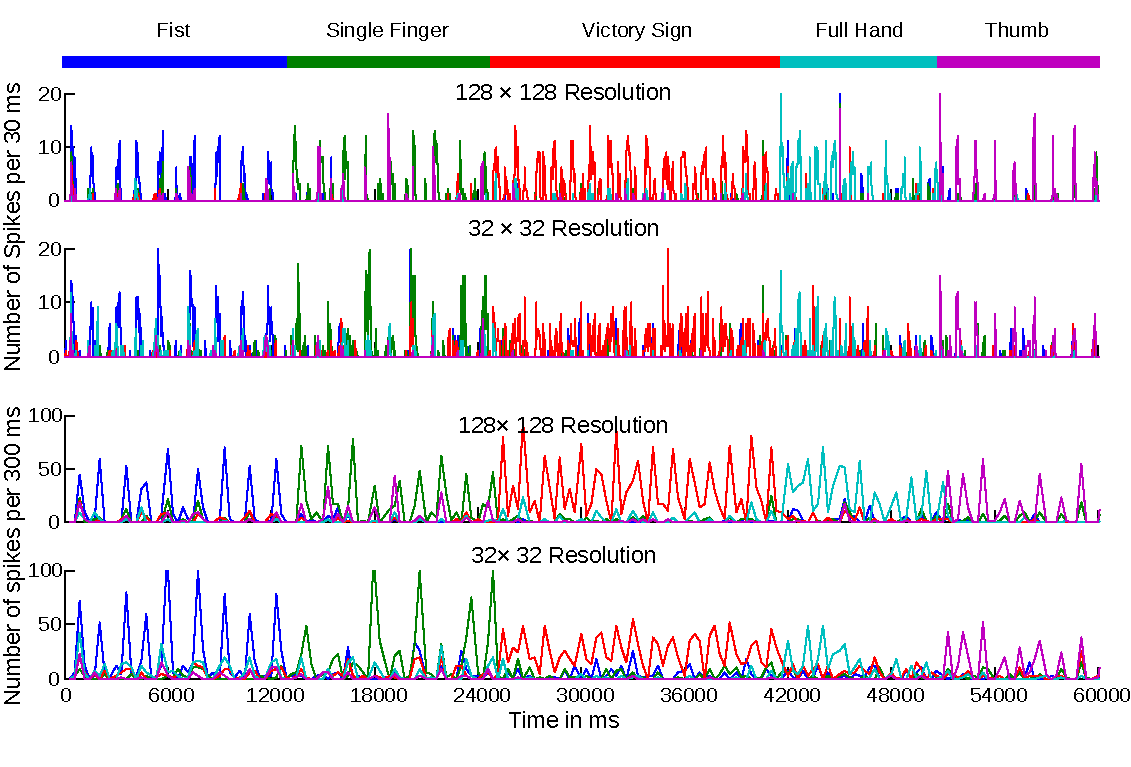
\includegraphics[width=\textwidth]{pics_icann/rateSpiNN.pdf}
	\caption{Real-time neural responses of two experiments on SpiNNaker with time to the same recorded postures.
	These two experiments only differ in input resolution.
	The result of the high input resolution test is plotted the first with a sample frame of 30~ms; 
	while the 3rd plot shows the same result with a sample frame of 300~ms.
	The other two plots refer to the smaller input resolution.
	Every point represents the over all number of spikes of a specific population (different colour) in a `frame'.
	}
	\label{fig:spikerec}
\end{figure}

Correspondingly, the spiking rates of each recognition population is sampled into frames (Fig.~\ref{fig:spikerec}) to make a comparison with the Matlab simulation. 
Each colour represents one recognition population, and the spike activity goes higher when the input posture matches the template. 
Firstly, the spike rates are sampled into 30~ms frames which is in accordance with the Matlab experiments.
In the Matlab simulation, the templates are trained with cut frames and so the test images are also fixed to the same length frames.
Otherwise, the recogniser will not work properly because of the replications of the moving posture.
Contrasting this, the spiking rates can be sampled to various frame lengths.
Thus, the other two plots in the figure illustrate the classification in a wider window of 300~ms.
From Table~\ref{tbl:srr}, the recognition and rejection rates are quantified as percentages.

Comparing with the results of Matlab simulation (Table~\ref{tbl:rsl}), the recognition rate is about 7.6\% lower at both high and low resolutions, and the rejection rate remains the same slightly above 75\%. 
However, by changing the frame length to 300~ms recognition rates reach (93.0\% for the larger network) or exceed (86.4\% for smaller network ) the Matlab simulation, meanwhile the rejection rates also drop dramatically by 26.0\% and 22.4\%.
This is in accordance with natural visual responses, which means, the longer an object shows, the more accurate the recognition will be.
Between the two network scales there is also a smaller gap in recognition rates as the window length grows, i.e. 8.9\% and 6.6\% respectively.
%Considering the cost and performance trade-off, with only 1/10th resources required, the small network, is acceptable and can be even improved after applying tracking and learning.
%Regarding the latency between the retinal input and the recognition, we compared the spiking peak of the Matlab simulation and the real-time SpiNNaker test.
%The overall latency is about 1150~ms from a posture being shown to its recognition. 

\begin{figure}
\centering
	\begin{subfigure}[t]{0.48\textwidth}
		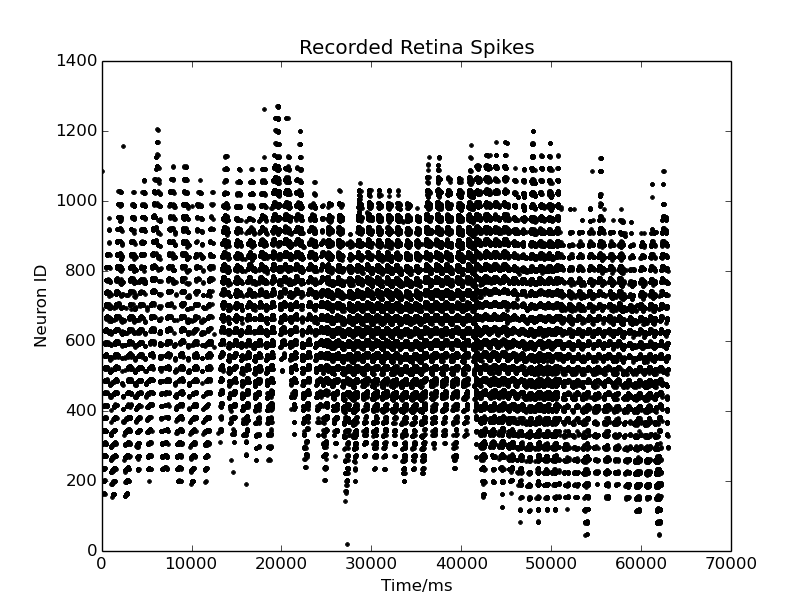
\includegraphics[width=\textwidth]{pics_icann/figure_r.png}
	    \caption{Retinal input population }
	    \label{fig:ssa}
	\end{subfigure}
	\begin{subfigure}[t]{0.48\textwidth}
		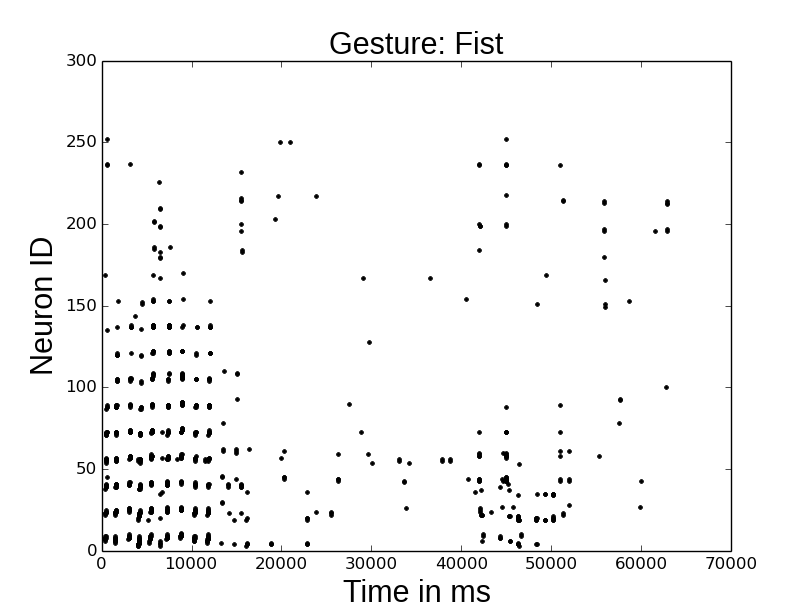
\includegraphics[width=\textwidth]{pics_icann/figure_1.png}
		\caption{Template matching population, `Fist'}
	    \label{fig:rec0}
	\end{subfigure}
	\\
	\begin{subfigure}[t]{0.48\textwidth}
		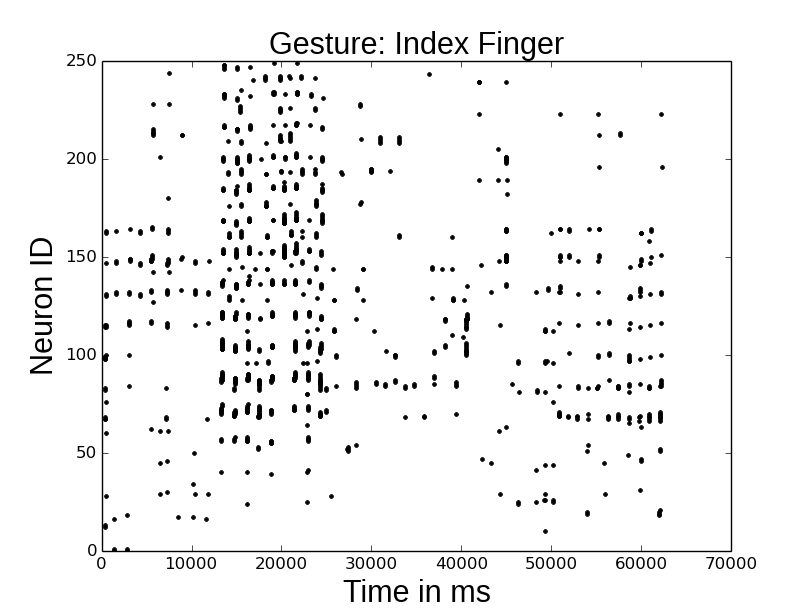
\includegraphics[width=\textwidth]{pics_icann/figure_2.png}
		\caption{Template matching population, `Index Finger'}
	    \label{fig:rec1}
	\end{subfigure}	
	\begin{subfigure}[t]{0.48\textwidth}
		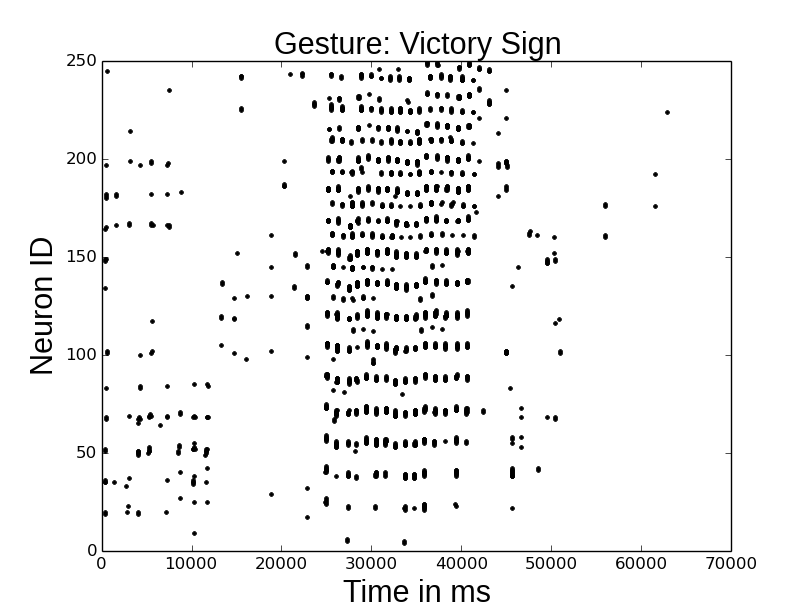
\includegraphics[width=\textwidth]{pics_icann/figure_3.png}
		\caption{Template matching population, `Victory Sign'}
	\end{subfigure}	
	\\
	\begin{subfigure}[t]{0.48\textwidth}
		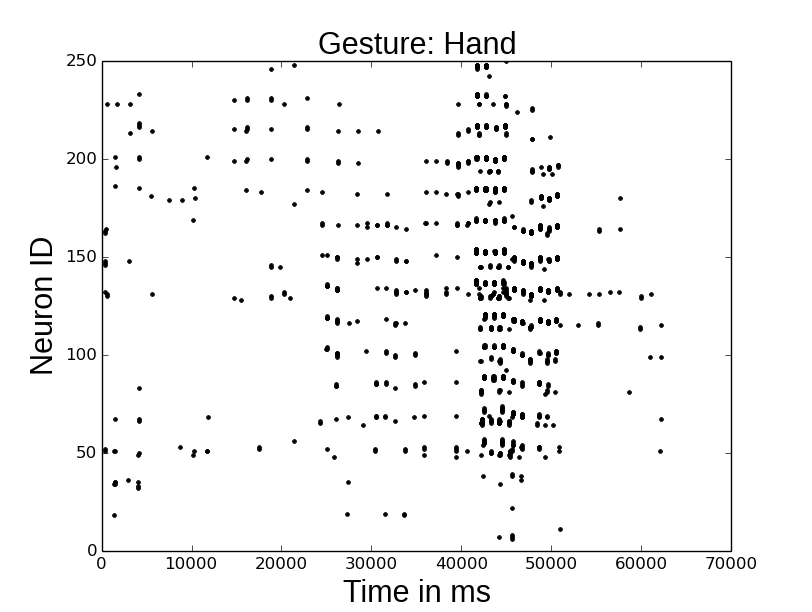
\includegraphics[width=\textwidth]{pics_icann/figure_4.png}
		\caption{Template matching population, `Full Hand'}
	    \label{fig:rec5}
	\end{subfigure}	
	\begin{subfigure}[t]{0.48\textwidth}
		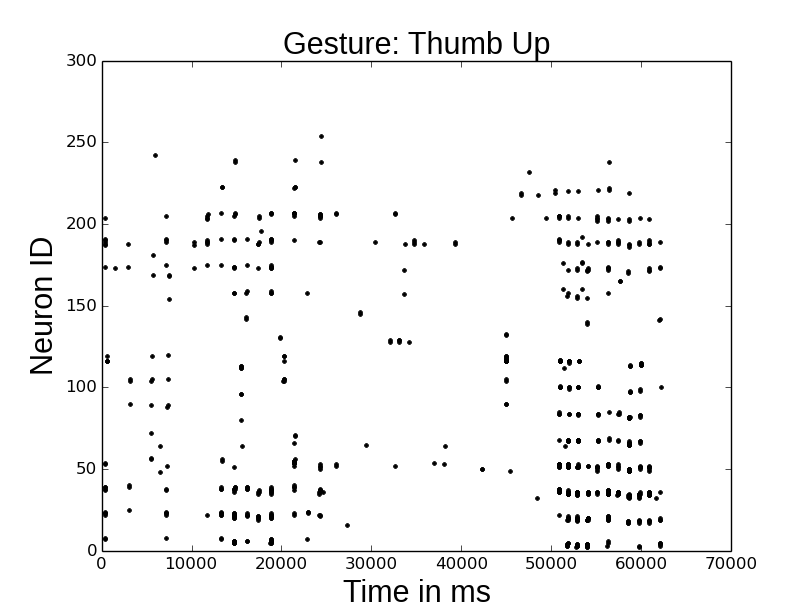
\includegraphics[width=\textwidth]{pics_icann/figure_5.png}
		\caption{Template matching population, `Thumb Up'}
	    \label{fig:rect}
	\end{subfigure}	
\caption{Spikes captured during the live recognition of the recorded retinal input with the resolution of 128$\times$128. }
\label{fig:rps}
\end{figure}
\begin{figure}
\centering
	\begin{subfigure}[t]{0.48\textwidth}
		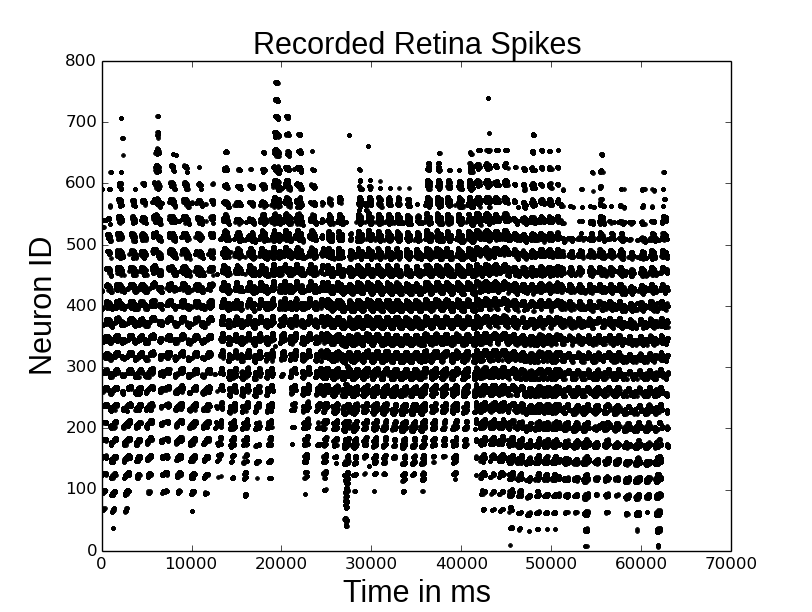
\includegraphics[width=\textwidth]{pics_icann/figure_32_r.png}
	    \caption{Retinal input population }
	    \label{fig:ssa32}
	\end{subfigure}
	\begin{subfigure}[t]{0.48\textwidth}
		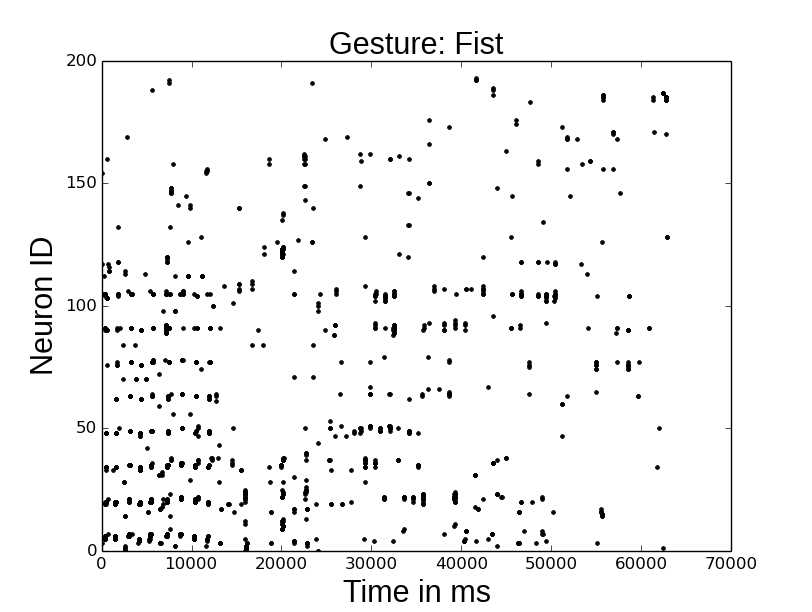
\includegraphics[width=\textwidth]{pics_icann/figure_32_1.png}
		\caption{Template matching population, `Fist'}
	    \label{fig:rec032}
	\end{subfigure}
	\\
	\begin{subfigure}[t]{0.48\textwidth}
		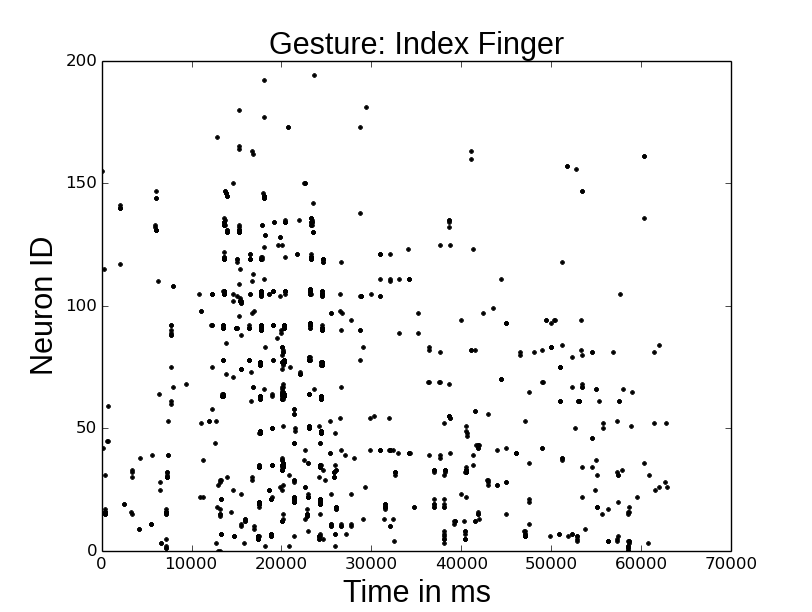
\includegraphics[width=\textwidth]{pics_icann/figure_32_2.png}
		\caption{Template matching population, `Index Finger'}
	    \label{fig:rec132}
	\end{subfigure}	
	\begin{subfigure}[t]{0.48\textwidth}
		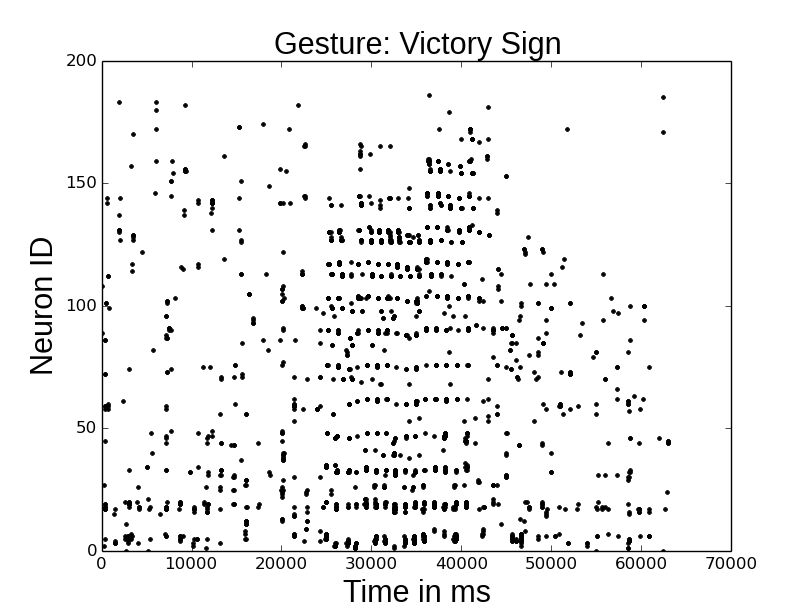
\includegraphics[width=\textwidth]{pics_icann/figure_32_3.png}
		\caption{Template matching population, `Victory Sign'}
	\end{subfigure}	
	\\
	\begin{subfigure}[t]{0.48\textwidth}
		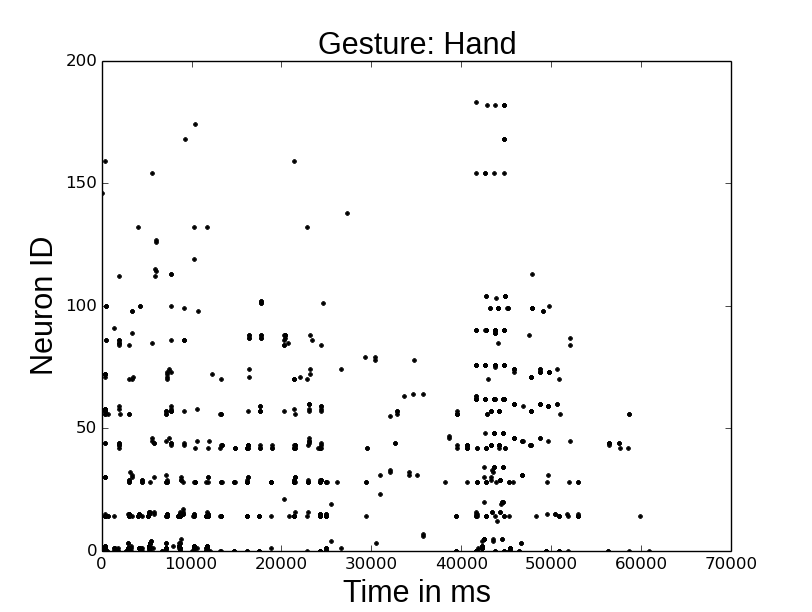
\includegraphics[width=\textwidth]{pics_icann/figure_32_4.png}
		\caption{Template matching population, `Full Hand'}
	    \label{fig:rec532}
	\end{subfigure}	
	\begin{subfigure}[t]{0.48\textwidth}
		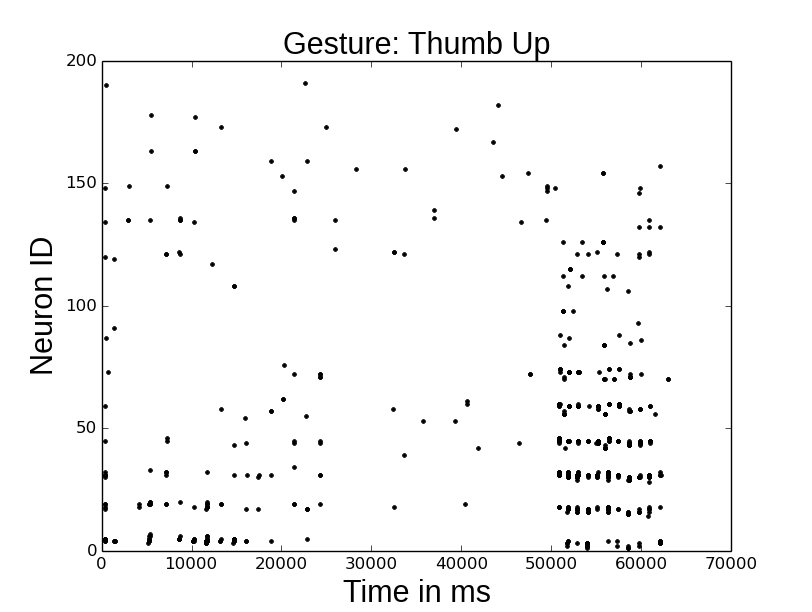
\includegraphics[width=\textwidth]{pics_icann/figure_32_5.png}
		\caption{Template matching population, `Thumb Up'}
	    \label{fig:rect32}
	\end{subfigure}	
\caption{Spikes captured during the live recognition of the recorded retinal input with the resolution of 32$\times$32. }
\label{fig:rps32}
\end{figure}
\begin{table}
\centering
\caption{Real-time recognition results on SpiNNaker in \%}
	\begin{tabular}{p{0.15\textwidth}|p{0.10\textwidth}<{\centering}|p{0.11\textwidth}<{\centering}|p{0.11\textwidth}<{\centering}|p{0.11\textwidth}<{\centering}|p{0.11\textwidth}<{\centering}}
		%Line 1
		\Xhline{1.2pt}
		    \multicolumn{2}{c|}{}	& \multicolumn{2}{c|}{\textbf{30~ms per frame}}  
		    & \multicolumn{2}{c}{\textbf{300~ms per frame}}
		    \\ \cline{3-6}
		%Line 2
		\multicolumn{2}{c|}{}	& \tabincell{c}{High \\ Resolution}
			& \tabincell{c}{Low \\ Resolution}
			& \tabincell{c}{High \\ Resolution}
			& \tabincell{c}{Low \\ Resolution}
			\\ \Xhline{1.2pt}
		%Line 3-4	
		\multirow{2}{*}{\tabincell{l}{\textbf{Fist}}}
			& Correct & 91.78	& 78.02	& 100	& 92.31
			\\ \cline{2-6}
			& Reject  & 82.78 & 78.54 	& 70.73	& 68.29
			\\ \hline
		%Line 5-6
		\multirow{2}{*}{\tabincell{l}{\textbf{Index Finger}}}
			& Correct & 78.25	& 78.25	& 88.24	& 72.22
			\\ \cline{2-6}
			& Reject & 80.46	& 73.56 	& 57.50	& 55.00
			\\ \hline
		%Line 7-8
		\multirow{2}{*}{\tabincell{l}{\textbf{Victory Sign} }}
			& Correct & 96.48	& 86.27	& 95.00	& 92.50
			\\ \cline{2-6}
			& Reject & 64.46	& 72.68 	& 28.57	& 28.57
			\\ \hline
		%Line 9-10
		\multirow{2}{*}{\tabincell{l}{\textbf{Full Hand}}}
			& Correct & 85.29	& 60.78	& 90.00	& 75.00
			\\ \cline{2-6}
			& Reject & 67.31	& 83.65 	& 35.48	& 61.29
			\\ \hline
		%Line 10-11
		\multirow{2}{*}{\tabincell{l}{\textbf{Thumb up}}}
			& Correct & 84.09	& 88.10	& 91.67	& 100
			\\ \cline{2-6}
			& Reject & 87.54	& 73.81 	& 66.67	& 66.67
			\\ \hline\hline
		\multirow{2}{*}{\tabincell{l}{\textbf{Average}}}
			& Correct & 87.18	& 78.28	& 92.98	& 86.41
			\\ \cline{2-6}
			& Reject & 76.51	& 76.45 	& 51.79	& 55.96
			\\ \hline
	\end{tabular}
	\label{tbl:srr}
\end{table}
